\subsection{Typicality Measures}\label{sec:typicality_measures}
Measuring typicality, i.e. how "dressy" a dress looks like, is a central aspect of the overall workflow. Having a consistent typicality measure allows to create supervision needed in the training of the manipulation method. Furthermore, it allows to validate the success of the manipulation ex-post quantitatively. Based on work by \cite{landwehr2011gut}, typicality is measured based on the cosine similarity of a product's features (i.e. its embedding) to a morph of the features of all products. With $f(\cdot)$ being any embedding model, the d-dimensional embedding for dress $D_i$ is calculated as $\boldsymbol{v}_i = f(D_i)$. Furthermore, the morph of all dresses is 
$$\boldsymbol{m} = \frac{1}{n} \sum_{i=1}^{n}\boldsymbol{v}_i,$$
with $\boldsymbol{v}_i \in \mathbb{R}^d$ and $\boldsymbol{m} \in \mathbb{R}^d$. Finally, the typicality measure for dress $D_i$ is 
$$typicality = cosine\_similarity(\boldsymbol{v}_i, \boldsymbol{m}) = \frac{\boldsymbol{v}_i \cdot \boldsymbol{m}}{|\boldsymbol{v}_i||\boldsymbol{m}|}.$$
In the first step, as a simple embedding model the pre-trained Vision Transformer (ViT) DINOv2 \citep{oquab2023dinov2} is used. More specifically, the "Base" version is used with a patch size of 14, i.e. the "ViT-B/14" configuration. The resulting embeddings are 1x768 dimensional. The authors claim that the representations are task-agnostic and general-purpose \citep[p.1]{oquab2023dinov2} and thus can be used for typicality analysis. While this approach may overfit to non-essential attributes or use shortcuts, the second embedding model I use aims to produce more holistic and robust representations. It does so by forcing the embedding model to learn multiple sub-embeddings, one for each relevant attribute of the dress. Thus, the decision about which features or attributes are important to represent a dress is not exclusively taken by the model as in the pure DINOv2 case but is defined ex-ante based on domain knowledge. The model starts with the simple DINOv2 embeddings and passes them through some fully connected layers. Afterwards, the embedding is split up into k subspaces $a_1,a_2,...,a_k$ by individual classification heads $C_1,C_2,...,C_k$, one for each attribute. The attributes selected consist of \textit{Color, Fabric, Fit, Neckline, Pattern, Collar, Length, Shape} and \textit{Sleeve Length}. Since the goal is to achieve disentangled sub-embeddings, a distance correlation (dCor) loss is added to the model training, enforcing the reduction of shared information across sub-embeddings. The distance correlation proposed by \cite{muller2024disentangling} measures nonlinear dependencies between vectors of any dimension and has been used by the authors for disentangled representation learning. The dCor loss is defined as 
$$\mathcal{L}_{dCor} = \sum_{i \neq j} \text{dCor}(a_i, a_j),$$
with 
$$\text{dCor}(a_1, a_2) = \sqrt{\frac{\text{dCov}^2(a_1, a_2)}{(\text{dVar}^2(a_1) \text{dVar}^2(a_2))^{1/2}}}.$$
Details about calculating $\text{dCov}^2$ and $\text{dVar}^2$ can be found in the original paper \citep[p.5]{muller2024disentangling} and in the appendix in equation \ref{eq:dcor_formula} to \ref{eq:last_dcor_formula}. A schematic overview of the disentangled embeddings model can be found in figure \ref{fig:disentangling_embeddings}.

\begin{figure}[ht!]
    \centering
    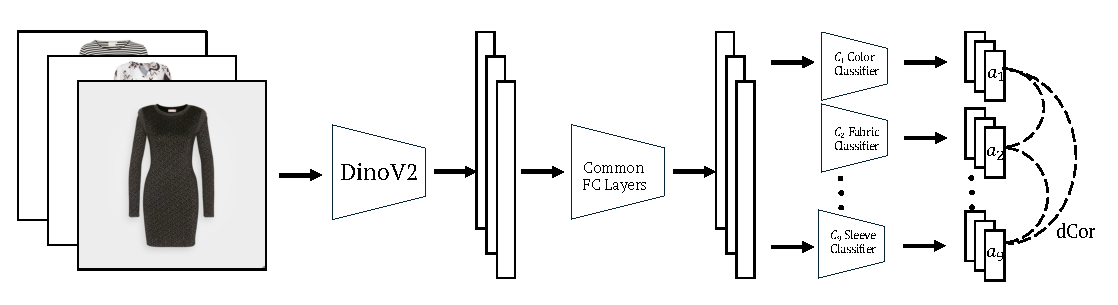
\includegraphics[width=1\linewidth]{Thesis/Method/assets/disentangling_embeddings-cropped.pdf}
    \caption[Disentangled Embeddings Model for Typicality]{Disentangled Embeddings Model for Typicality: \textit{Initial DINOv2 embeddings are divided into subspace embeddings $a_1,a_2,...,a_k$ by classifiers. Disentanglement is forced by a distance correlation loss between all sub-embeddings}}
    \label{fig:disentangling_embeddings}
\end{figure}

Each subspace embedding in this disentangled embedding model is 1x256 dimensional and thus the complete embedding, which is a concatenation of all subspace embeddings, has dimension 1x2304. Apart from the complete concatenation, I also construct embeddings that exclude one subspace at a time. This might be e.g. all subspace embeddings except the \textit{Color} subspace such that the model can calculate the typicality of a dress but does not take the \textit{Color} attribute of the dress into account.


It is important to note that both typicality measures are learned on the reconstructed images using the e4e inversion \citep{tov2021designing}. Thus, the embeddings for each dress, as well as the morphs, are calculated based on the respective reconstructions. Training the typicality measure on real images and using generated images at test time holds potential for problems. Although the reconstructions are very accurate, pixel values and low-level image features might differ between the generator outputs and the real image distribution, thus introducing possible mismatches in the typicality calculations.